\subsection{Consequences from changing the template}
\label{sec:conseq}

In the original template the moving window integration filter computed an average of the last 30 values. Our chosen implementation averages the last 32 elements instead. The reason for this choice is that division is a very heavy computation\footnote{The data values peak at $\approx$ 4700. Assuming the previous 30 values are $\geq$ 2000, calculating the average after a peak by integer division would take $\frac{60000}{30} = 2000$ cycles of computation for our particular data set.}. When assessing 32 elements instead, the sum can be bit shifted 5 places. This speeds the computation up significantly as the bit-wise command only takes one clock cycle. \\
\\
Using $N=32$ instead of $N=30$ when averaging, one would expect that the filtered signal profile is flatter, and slightly delayed. The reason is that more data points are included in the sum, and an ECG signal consists mostly of short high-value pulses separated by long low-value regions. When encountering a peak, more low values are initially kept in the sum. After a peak, the sum decreases slower, as more high values are kept.
\\
The two sets of filtered data are calculated in the C program from assignment 1, and shown in figure \ref{fig:points30}. 
 
\begin{figure}[H]
\centering
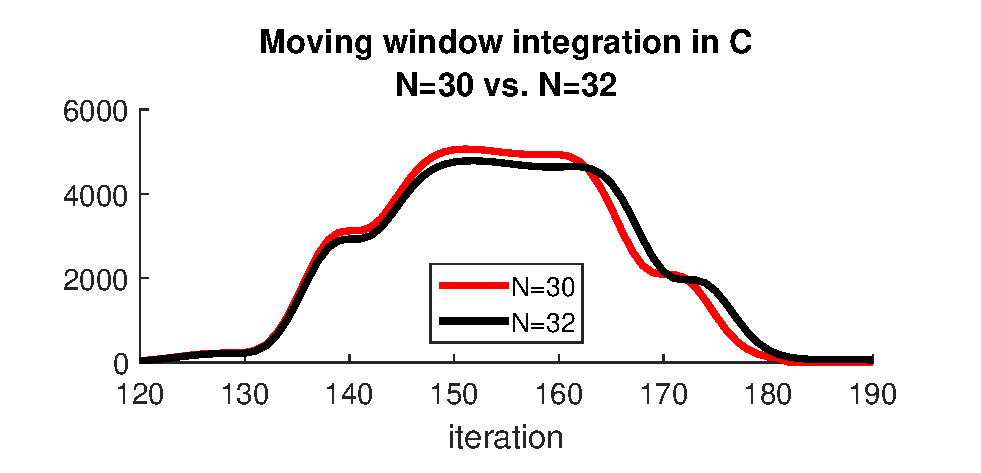
\includegraphics[width=1.0\textwidth]{2Implementation/fig/points30.eps}
\caption{Graph showing peak profiles when the moving window integration filter is applied with $N=30$ and $N=32$, respectively.}
\label{fig:points30}
\end{figure}

As expected for $N=32$, the filtered signal has a lower value on the left and top side of the peak. Filtered values after the peak also decrease slower. as expected.\\
%The far side of the peak results in larger values, which is explained by the last 32 data points now being on the of the peak. \\
\\
An overall assessment of the peak profile is that its shape and dominant features are nicely maintained. Meaning that the consequence of changing the algorithm is minimal. With $N=32$, the C program finds the same Rpeaks as with $N=30$. This is checked in figure \ref{fig:comparingPeaksC30C32}.

\begin{figure}[H]
\centering
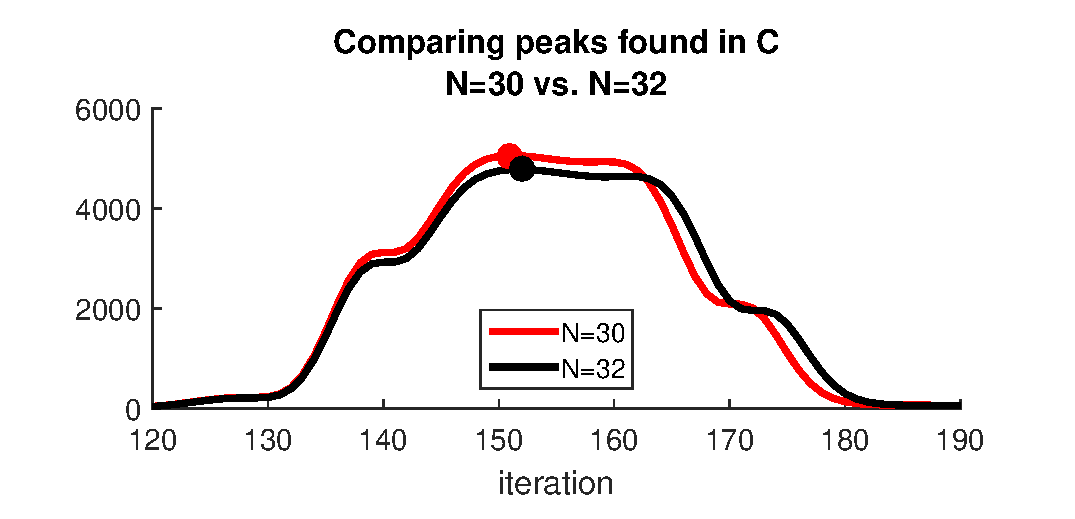
\includegraphics[width=1.0\textwidth]{2Implementation/fig/comparingPeaksC30C32.eps}
\caption{Following figure \ref{fig:points30}, this graph shows the found Rpeak when doing peak detection from assignment 1.}
\label{fig:comparingPeaksC30C32}
\end{figure}

As figure \ref{fig:comparingPeaksC30C32} shows, when running the peak detection from assignment 1, the Rpeak is found correctly. We performed additional tests to verify that we find the same peaks with $N=32$ as with $N=30$. For a complete and statistical comparison between Rpeaks, see appendix \ref{sec:AppComparingPeaks}. 